\documentclass[emulatestandardclasses]{scrartcl}
\usepackage{graphicx}
\usepackage{color}
\usepackage[ngerman]{babel}
\usepackage{hyperref}
\usepackage{fullpage}
\usepackage{calc} 
\usepackage{enumitem}
\usepackage{titlesec}
\newcommand{\todo}[1]{\textcolor{red}{TODO: #1}\PackageWarning{TODO:}{#1!}}
\date{\vspace{-3ex}}
\begin{document}

\title{
	\includegraphics*[width=0.75\textwidth]{ErstesSem/images/hu_logo.png}\\
	\vspace{24pt}
	Heideggers Sein und Zeit, Heideggers Schwarze Hefte}
\subtitle{Proseminar SS 17\\
          Prof. Dr. Babette Babich\\
          Philosophische  \\ 
          Humboldt Universit"at zu Berlin}
\author{Lennard Wolf\\
        \small{\href{mailto:lennard.wolf@student.hu-berlin.de}{lennard.wolf@student.hu-berlin.de}}}
\maketitle
\begin{abstract}

In der Vorlesung wird es um Heideggers Sein und Zeit sowie um den ersten (und möglicherweise weitere Bände) seiner jüngst veröffentlichten sogenannten Schwarzen Hefte gehen. Abgesehen davon, dass die Debatte um seinen Antisemitismus im Zusammenhang sowohl der damaligen politischen Situation als auch des gegenwärtigen Kontextes im Blick steht, werden wir beide Texte, den veröffentlichten (Sein und Zeit) sowie den bis vor drei Jahren unpublizierten Nachlass Heideggers zusammenlesen. Auf diese Weise kann man zu einem besseren Verständnis sowohl seines philosophischen Entwurfes gelangen als auch der üblich gewordenen Aufteilung seines Denkens in einen Heidegger I vor der “Kehre” und einen Heidegger II nach der “Kehre”. Das schließt Fragen ein wie die nach dem Sein, nach der Sprache, aber auch jene nach der modernen Wissenschaft und Technik. Weitere Problemfelder werden das augenblickliche Klima des Heidegger-Skandals sein, Fragen in Bezug auf die analytische, die kontinentale sowie die digitale Philosophie und ihren jeweiligen Niederschlag hinsichtlich der Übermittlung von Texten und Lektürestrategien wie Überlegungen zu bis heute aktuellen Aspekten von Heideggers Kritik, wie etwa seine Kritik der Medien.
Die Veranstaltung wird neben der Vorlesung ausdrücklich auf Diskussion ausgerichtet. Gleichzeitig wird es die Gelegenheit geben, sich mit Beginn des Semesters in einem begleitenden Blockseminar intensiv mit Sein und Zeit auseinanderzusetzen. Für das Ende des Semesters ist ein ergänzendes Kolloquium über die Schwarzen Hefte geplant. Die Diskussionen finden auf Englisch und auf Deutsch statt.
\end{abstract}
\newpage

\tableofcontents
\listoffigures
\newpage


\section{Einf"uhrungssitzung\\(18.05.17)}

\subsection{Organisatorisches}

\begin{itemize}
  \item Wir brauchen Heidegger-Philologie, sowie Hermeneutik, die es bisher nicht gibt
  \item 
\end{itemize}


\begin{description}[leftmargin=!,labelwidth=\widthof{\bfseries Erscheinendes Bewusstsein}]
  \item[Reines Sein]
  \item[Allgemeines] Etwas das durch Negation ist; es ist das Wahre der sinnlichen Gewissheit
\end{description}


\newpage
\section{"Uber den Professor}
Prof. Mustermann ist..


%\begin{figure}[h]
%	\centering
%	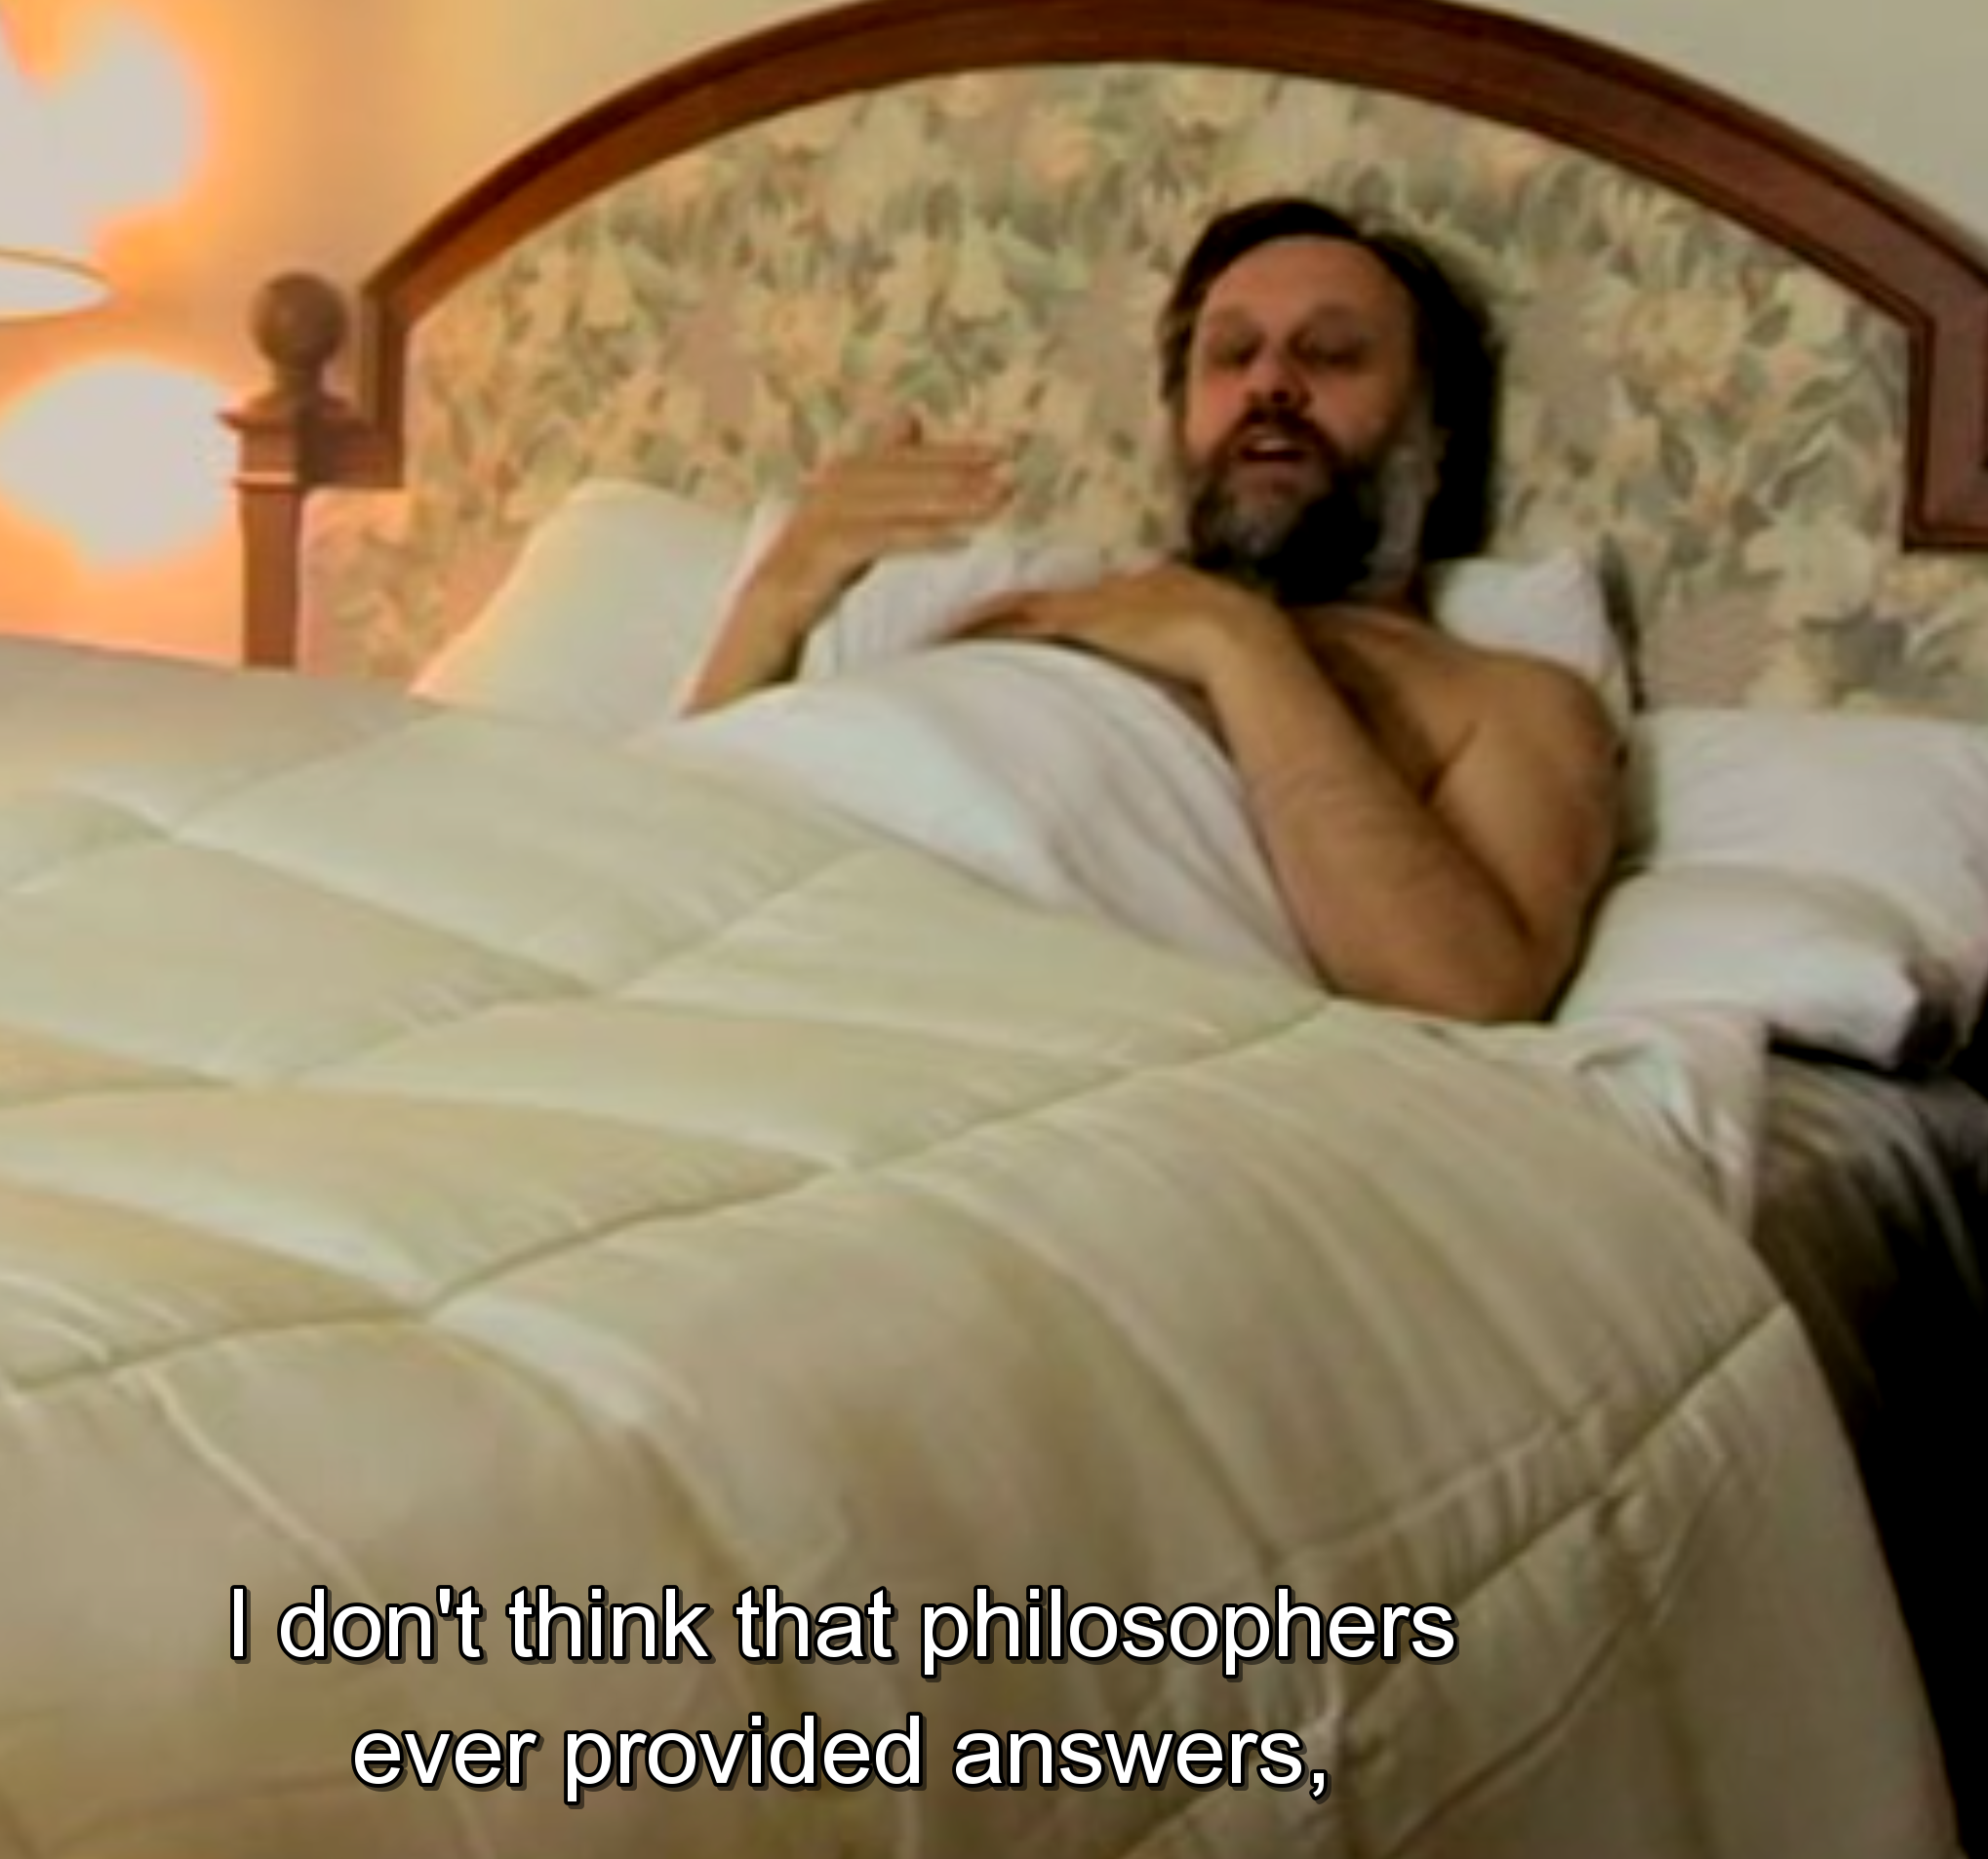
\includegraphics[width=0.5\textwidth]{images/template.png}
%	\caption{Template Bild}
%	\label{fig:template}
%\end{figure}

\end{document}
